%% LyX 1.1 created this file.  For more info, see http://www.lyx.org/.
%% Do not edit unless you really know what you are doing.
\documentclass[12pt,english]{amsart}
\usepackage[T1]{fontenc}
\usepackage[latin1]{inputenc}
\usepackage{fancyhdr}
\pagestyle{fancy}
\usepackage{babel}
\usepackage{color}
\makeindex
\usepackage{graphics}
\usepackage{varioref}

\makeatletter

%%%%%%%%%%%%%%%%%%%%%%%%%%%%%% LyX specific LaTeX commands.
\providecommand{\LyX}{L\kern-.1667em\lower.25em\hbox{Y}\kern-.125emX\@}

%%%%%%%%%%%%%%%%%%%%%%%%%%%%%% Textclass specific LaTeX commands.
 \theoremstyle{plain}    
 \newtheorem{thm}{Theorem}[section]
 \numberwithin{equation}{section} %% Comment out for sequentially-numbered
 \numberwithin{figure}{section} %% Comment out for sequentially-numbered
 \theoremstyle{plain}    
 \newtheorem{cor}[thm]{Corollary} %%Delete [thm] to re-start numbering
 \theoremstyle{plain}    
 \newtheorem{lem}[thm]{Lemma} %%Delete [thm] to re-start numbering
 \theoremstyle{plain}    
 \newtheorem{prop}[thm]{Proposition} %%Delete [thm] to re-start numbering
 \theoremstyle{definition}
 \newtheorem{defn}[thm]{Definition}
 \theoremstyle{definition}
  \newtheorem{example}[thm]{Example}
 \newcommand{\lyxaddress}[1]{
   \par {\raggedright #1 
   \vspace{1.4em}
   \noindent\par}
 }

%%%%%%%%%%%%%%%%%%%%%%%%%%%%%% User specified LaTeX commands.
\usepackage {graphicx}


\usepackage{epsfig}
\usepackage{amsmath,amssymb}
\usepackage{pslatex}
\usepackage{color}

 
 \definecolor{veryblackblue}{rgb}{0.0,0.0,0.1}
 \usepackage[pdftex,urlcolor=webblackblue,colorlinks=true,citecolor=blue,linkcolor=webblackblue]{hyperref}
 \pdfinfo{
            /Title      (Mathematics 2023 - Infinite Series I)
            /Author     (Daniel Lemire)
            /Subject    (A document on series for the course topics from advanced calculs offered at Acadia University.)
            /Keywords   ( series, convergence, Taylor, ratio test, cauchy sequences)
          }


\topmargin  = 0pt
\headheight = 0pt
\headsep    = 0pt

\voffset    = 0in
\hoffset    = 0in
\textheight = 230mm
\textwidth  = 164mm

\evensidemargin = 0pt
\oddsidemargin  = 0pt

\pagestyle{empty}
\usepackage{float}

%% Background of blue palette
 \definecolor{webblackblue}{rgb}{0.0,0.0,0.2}
 \definecolor{webblue}{rgb}{0.0, 0.0, 0.6}

%% Background of red palette
 \definecolor{webblackred}{rgb}{0.2,0.0,0.0}
 \definecolor{webred}{rgb}{0.6,0.0,0.0}

%% Background of green palette
 \definecolor{webblackgreen}{rgb}{0.0,0.2,0.0}                                   
 \definecolor{webgreen}{rgb}{0.0,0.6,0.0} 

%% Background of magenta palette
 \definecolor{webblackmagenta}{rgb}{0.14,0.0,0.14}                                   
 \definecolor{webmagenta}{rgb}{0.42,0.0,0.42} 

%% Background of cyan palette
 \definecolor{webblackcyan}{rgb}{0.0,0.14,0.14}                                   
 \definecolor{webcyan}{rgb}{0.0,0.42,0.42} 

%% Background of yellow pallete
 \definecolor{webblackyellow}{rgb}{0.14,0.14,0.0}                                   
 \definecolor{webyellow}{rgb}{0.85,0.85,0.0} 

 \definecolor{webdarkgray}{rgb}{0.2,0.2,0.2}

 \definecolor{webgray}{rgb}{0.75,0.75,0.75}
 \definecolor{weborange}{rgb}{1.0, 0.6, 0.0}

\renewcommand\labelenumi{\textcolor{webdarkgray}{\arabic{enumi}.}}
\newcommand{\setenumi}[1]{#1.\setcounter{enumi}{#1}}
\usepackage{dsfont}

\makeatother
\begin{document}

\title{Mathematics 2023 - Infinite Series I\\
Acadia University}


\lyxaddress{Copyright 1998 F. Chipman \\
Revised 1999 T. Archibald\\
Revised 2001 D. Lemire}

\maketitle
\tableofcontents{}


\section{Taylor Polynomials}

We recall the idea of a Taylor polynomial used as a local approximation
to a function. By local, we mean that the approximation is perfect
at some point \( x=a \). We then say the polynomial is found \char`\"{}at\char`\"{}
or \char`\"{}about\char`\"{} this point.

Given a function \( f(x) \) that is continuous on some interval \( I \)
containing the point \( x=a \), and has \char`\"{}enough\char`\"{}
continuous derivatives on \( I \), the Taylor polynomial\index{Taylor polynomial}
of degree \( n \) for \( f(x) \), expanded about \( x=a \), is
given by

\[
P_{n}(x)=f(a)+f\, '(a)(x-a)+\frac{f\, ''(a)}{2\, !}(x-a)^{2}+\frac{f\, ^{(3)}\left( a\right) }{3\, !}(x-a)^{3}+\cdots +\frac{f\, ^{(n)}\left( a\right) }{n\, !}(x-a)^{n}\]


(Recall that \( n\, !=1\cdot 2\cdot 3\cdot 4\cdot \cdots \cdot n \)
is called {}``\( n \)~factorial'' and is the product of the first
\( n \) counting numbers. The symbol \( f^{(n)}(x) \) is the \( n^{th} \)
derivative of \( f(x) \).)

\begin{example}
Consider the function \( f(x)=e^{x} \) about the point \( x=0 \).
Because all of the derivatives of \( e^{x} \)are the same, and have
a value of 1 at \( x=0 \), we have\[
e^{x}\approx P_{n}(x)=1+x+\frac{x^{2}}{2\, !}+\frac{x^{3}}{3\, !}+\frac{x^{4}}{4\, !}+\cdots +\frac{x^{n}}{n\, !}\]
Notice that \( P_{1}(x)=1+x \) is just the usual linear approximation
to \( e^{x} \) at \( x=0 \), and \( P_{2}(x)=1+x+x^{2}/2! \) is
the quadratic approximation. Taylor polynomials are just the natural
extension of these approximations to higher degrees.
\end{example}
~

\begin{example}
\label{lnexample}Consider the function \( f(x)=\ln (x) \). Since
the function is undefined at \( x=0 \), we must choose some other
point for expansion, say \( x=1 \). To find the polynomial of degree
\( n \), we calculate the coefficients and look for a pattern.\[
{\begin{array}{*{20}c}
{f(x)=\ln (x),}\hfill  & {f(1)=0,}\hfill  &  &  &  & \\
{f\, '(x)=x^{-1},}\hfill  & {f\, '(1)=1,}\hfill  &  &  &  & \\
{f\, ''(x)=-x^{-2},}\hfill  & {f\, ''(x)=-1,}\hfill  &  &  &  & \\
{f\, ^{(3)}(x)=2x^{-3},}\hfill  & {f\, ^{(3)}(1)=2,}\hfill  &  &  &  & \\
{f\, ^{(4)}(x)=-3\cdot 2\cdot x^{-4},}\hfill  & {f\, ^{(4)}(1)=-3\, !}\hfill  &  &  &  & \\
{f\, ^{(5)}(x)=4\, !\, x^{-5},}\hfill  & {f\, ^{(5)}(1)=4\, !,}\hfill  &  &  &  & \\
\vdots \hfill  & \vdots \hfill  &  &  &  & \\
{f\, ^{(n)}(x)=\pm (n-1)!x^{-n},}\hfill  & {f\, ^{(n)}(1)=\pm (n-1)!}\hfill  &  &  &  & \\
\hfill  & \hfill  &  &  &  & \\

\end{array}}\]
 This gives\[
P_{n}(x)=(x-1)-\frac{(x-1)^{2}}{2}+\frac{2(x-1)^{3}}{3\, !}-\frac{3\, !(x-1)^{4}}{4\, !}+\cdots +\frac{(-1)^{n-1}(n-1)\, !(x-1)^{n}}{n\, !}.\]
Using the fact that \( \frac{(n-1)\, !}{n\, !}=\frac{1}{n} \) (why
??), we have\[
P_{n}(x)=(x-1)-\frac{(x-1)^{2}}{2}+\frac{(x-1)^{3}}{3\, }-\frac{(x-1)^{4}}{4\, }+\cdots +\frac{(-1)^{n-1}(x-1)^{n}}{n}.\]
Since we are considering the Taylor polynomials as approximations
of \( f(x) \) near the point \( x=a \), it is interesting to see
how closely the polynomials we have derived resemble the functions.
The fast way to do this is to use Maple. The two important commands
here are \char`\"{}taylor\char`\"{} to generate the series for a given
function; and \char`\"{}convert\char`\"{} which changes the series
(which is thought of as an infinitely long polynomial) to the finite
Taylor polynomial we want.
\end{example}
~

\begin{example}
{\raggedright Here is a Maple session in which we use the {}``taylor''
command to generate the first 5 approximations \( P_{0}(x),P_{1}(x),\ldots ,P_{4}(x) \),
and then plot them all on the same plot. I have used a \char`\"{}do\char`\"{}
statement to permit me to do several operations\par}

{\raggedright \textsf{\textcolor{blue}{> f:=exp(x); a:=0;}}\\
\textsf{\textcolor{blue}{f := exp(x)}}\\
\textsf{\textcolor{blue}{a := 0}}\\
\textsf{\textcolor{blue}{> for n from 0 to 4 do p{[}n{]}:=convert(taylor(f,x=a,n+1),polynom);
od;}}\\
\textsf{\textcolor{blue}{p{[}0{]} := 1}}\\
\textsf{\textcolor{blue}{p{[}1{]} := 1 + x}}\\
\textsf{\textcolor{blue}{p{[}2{]} := 1 + x + 1/2 x}}\textcolor{blue}{\( ^{2} \)}\textsf{\textcolor{blue}{}}\\
\textsf{\textcolor{blue}{p{[}3{]} := 1 + x + 1/2 x}} \textcolor{blue}{\( ^{2} \)}
\textsf{\textcolor{blue}{+ 1/6 x}}\textcolor{blue}{\( ^{3} \)}\textsf{\textcolor{blue}{}}\\
\textsf{\textcolor{blue}{p{[}4{]} := 1 + x + 1/2 x}}\textcolor{blue}{\( ^{2} \)}
\textsf{\textcolor{blue}{+ 1/6 x}}\textcolor{blue}{\( ^{3} \)} \textsf{\textcolor{blue}{+
1/24 x}}\textcolor{blue}{\( ^{4} \)}\textsf{\textcolor{blue}{}}\\
\textsf{\textcolor{blue}{> plot({[}f,p{[}k{]}\$k=0..4{]},x=-2..2,colour=black);}}
\centerline{\resizebox*{0.45\columnwidth}{!}{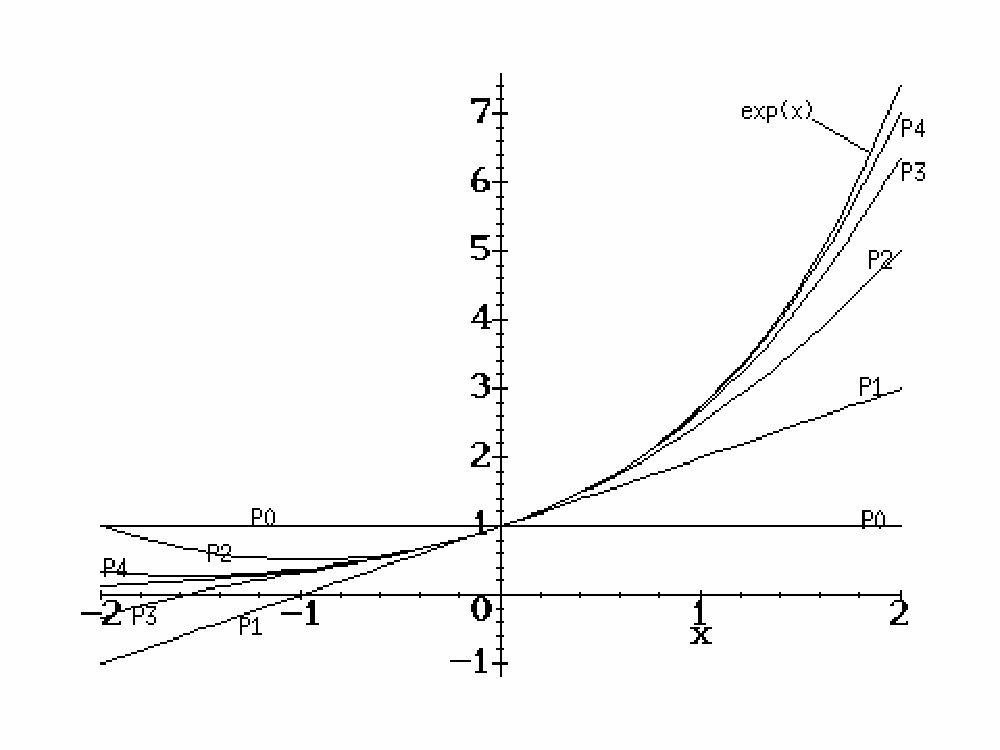
\includegraphics{series1.pdf}} }
\label{fig1}\\
Note that for \( x>0 \) the approximations all lie below \( e^{x} \),
but seem to get closer to \( e^{x} \) as the degree of the polynomial
increases. In fact, on the interval {[}-1, 1{]} it is hard to distinguish
\( P_{4}(x) \) from the function \( e^{x} \).\par}
\end{example}
~

\begin{example}
{\raggedright Now let's return to Example \ref{lnexample}, where
\( f(x)=\ln (x) \) and we expanded about \( a=1 \). It is just a
matter of replacing \( f \) with this new function in the Maple commands
we used above:\par}

{\raggedright \textsf{\textcolor{blue}{> f:=ln(x); a:=1;}}\\
\textsf{\textcolor{blue}{> for n from 0 to 4 do: p{[}n{]}:=convert(taylor(f,x=a,n+1),polynom);
od;}}\\
\textsf{\textcolor{blue}{f := ln(x)}}\\
\textsf{\textcolor{blue}{a := 1}}\\
\textsf{\textcolor{blue}{p{[}0{]} := 0}}\\
\textsf{\textcolor{blue}{p{[}1{]} := x - 1}}\\
\textsf{\textcolor{blue}{p{[}2{]} := x - 1 - 1/2 (x - 1)}}\textcolor{blue}{\( ^{2} \)}\textsf{\textcolor{blue}{}}\\
\textsf{\textcolor{blue}{p{[}3{]} := x - 1 - 1/2 (x - 1)}}\textcolor{blue}{\( ^{2} \)}\textsf{\textcolor{blue}{+
1/3 (x - 1)}}\textcolor{blue}{\( ^{3} \)}\textsf{\textcolor{blue}{}}\\
\textsf{\textcolor{blue}{p{[}4{]} := x - 1 - 1/2 (x - 1)}}\textcolor{blue}{\( ^{2} \)}
\textsf{\textcolor{blue}{+ 1/3 (x - 1)}}\textcolor{blue}{\( ^{3} \)}
\textsf{\textcolor{blue}{- 1/4 (x - 1)}}\textcolor{blue}{\( ^{4} \)}\textsf{\textcolor{blue}{}}\\
\textsf{\textcolor{blue}{> plot({[}f,p{[}k{]}\$k=0..4{]},x=0..2,colour=black);}}\par}

{\raggedright \centerline{\resizebox*{0.45\columnwidth}{!}{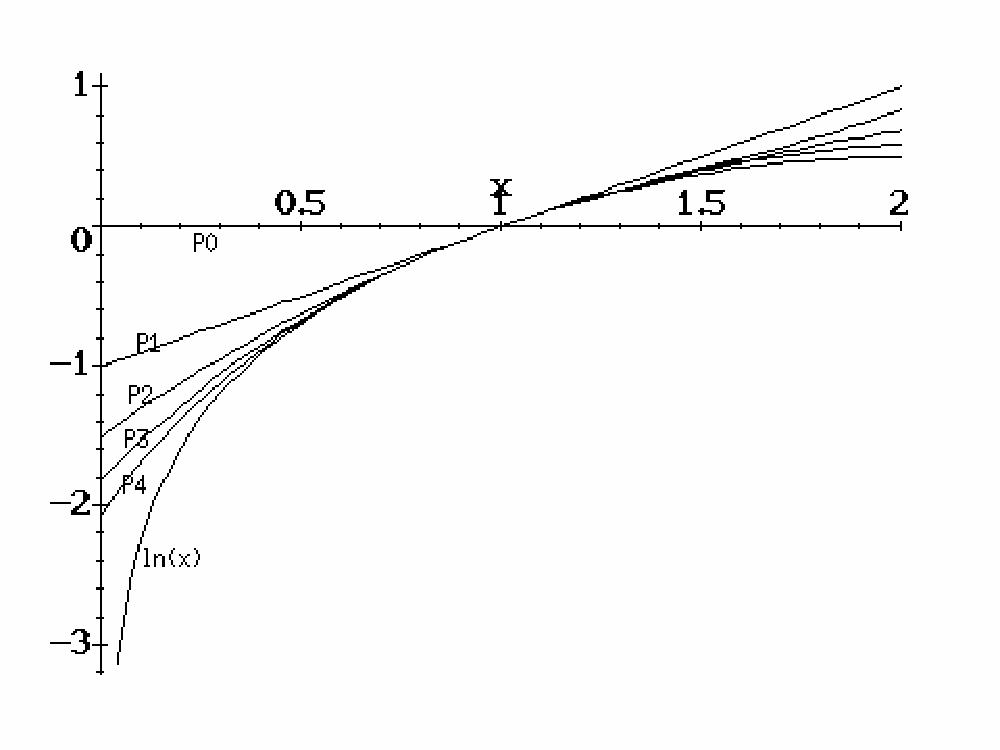
\includegraphics{series2.pdf}} }
\label{fig2}\par}

{\raggedright Once again it appears that the on the interval shown,
the polynomials get closer to the function \( f(x)=\ln (x) \) as
the degree of the polynomials increase. However. if we look a little
further away from \( x=1 \) by extending the interval from \( x=0 \)
to \( x=3 \), we get quite a different picture:\par}

{\raggedright \textsf{\textcolor{blue}{> plot({[}f,p{[}k{]}\$k=0..4{]},x=0..3,colour=black);}}\par}

{\raggedright \centerline{\resizebox*{0.45\columnwidth}{!}{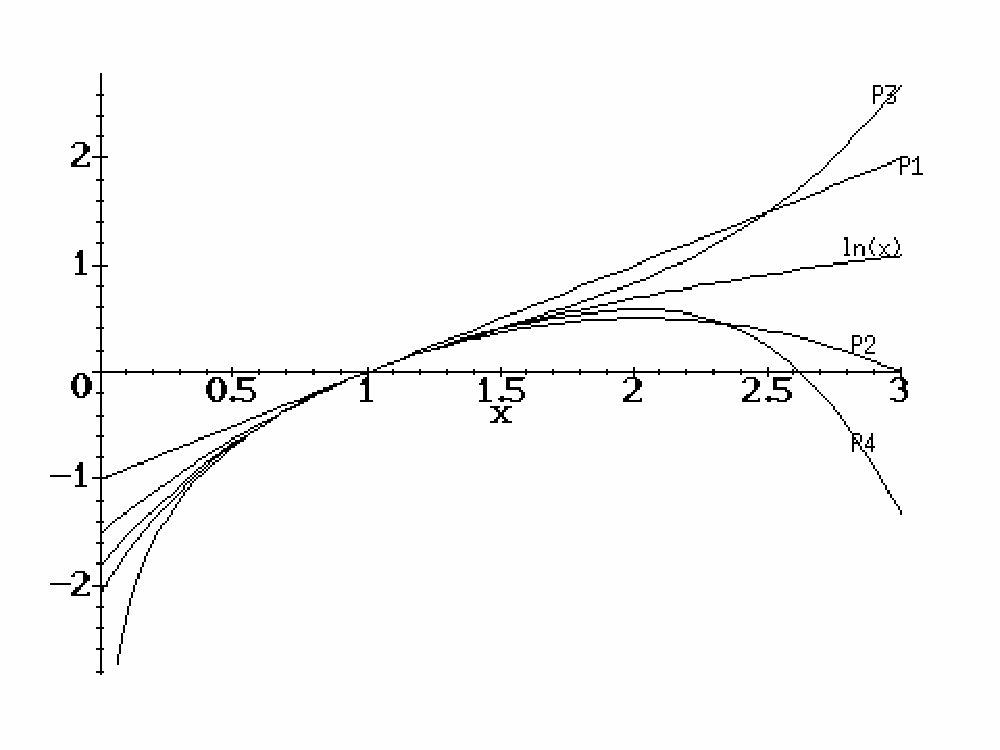
\includegraphics{series3.pdf}} }
\label{fig3}\par}

{\raggedright Here we note that on the interval {[}2, 3{]} things
do not seem to be going very well for our Taylor polynomials, viewed
as approximations to \( \ln (x) \). At \( x=3 \) it looks as if
the polynomials no longer approach \( \ln (x) \), but become further
away as the degree of the polynomial increases. In fact, we shall
show later that these particular approximations for \( \ln (x) \)
are valid only over the interval (0, 2{]}.\par}
\end{example}
We now pause to explain the Maple\index{Maple} commands we have used
in the above examples. \textsf{}\textsf{\textcolor{blue}{taylor(f,x=a,n);}}
 produces an infinite Taylor series for f expanded about \( x=a \),
and displays the first \( n \) terms of that series. Here \( f \)
must be what Maple calls an expression (in \( x \)), rather than
a function defined using the arrow (e.g. \( f:=\sin (x) \) is all
right, but \( f:=x->\sin (x) \) won't work). The result is a Taylor
polynomial of degree \textbf{\( n-1 \)} followed by the symbol \textsf{+
O((x-a)}\( ^{n} \)\textsf{).} This symbol stands for all the remaining
terms of the series, and indicates they all contain a factor \textsf{(x-a)}\( ^{n} \).
(We read the symbol \textsf{O((x-a)}\( ^{n} \)\textsf{)} as \char`\"{}
terms of order (x-a)\( ^{n} \)\char`\"{}.) Note that the first \( n \)
terms displayed give a polynomial of degree \( n-1 \), since the
first term is degree 0, the second degree 1, etc.

Of course, in our example we wanted Taylor polynomials, not Taylor
series. The \textsf{\textcolor{blue}{convert}} command will convert
a Taylor series to a Taylor polynomial by deleting the \textsf{O((x-a)}\( ^{n} \)\textsf{)}
term at the end. Thus if we wanted the Taylor polynomial of degree
5 for the function \( f(x)=\sin (x) \) expanded about \( x=a=0 \),
we would use the Maple command\textsf{\textcolor{blue}{}}\\
\textsf{\textcolor{blue}{> t5:=taylor(sin(x),x=0,6);}}\\
\textsf{\textcolor{blue}{t5 := x - 1/6 x}}\textcolor{blue}{\( ^{3} \)}
\textsf{\textcolor{blue}{+ 1/120 x}}\textcolor{blue}{\( ^{5} \)}
\textsf{\textcolor{blue}{+ O(x}} \textcolor{blue}{\( ^{6} \)}\textsf{\textcolor{blue}{)}}\\
\textsf{\textcolor{blue}{> p5:=convert(t5,polynom);}}\\
\textsf{\textcolor{blue}{p5 := x - 1/6 x}}\textcolor{blue}{\( ^{3} \)}
\textsf{\textcolor{blue}{+ 1/120 x}}\textcolor{blue}{\( ^{5} \)}\\
If these polynomial approximations are to be of any practical value,
we must be able to determine how accurately they approximate the given
function. We now consider this problem.


\section{How accurate are Taylor polynomials as approximations? }

Since \( P_{n}(x)\approx f(x) \) for \( x \) near the point \( x=a \),
we now investigate ways to estimate the size of the error \( \left| {f(x)-P_{n}(x)}\right|  \)
at any point \( x \). 

\begin{thm}
(Taylor) Let \( f(x) \) have \( n+1 \) continuous derivatives on
the interval \textsf{\textbf{\( I \)}} containing the point \( x=a \).
Let \( P_{n}(x) \) be the Taylor polynomial of degree \( n \) for
\( f(x) \) expanded about the point \( x=a \). Then for any point
\( x \) on the interval \textsf{\textbf{\( I \)}}, we have\[
f(x)-P_{n}(x)=\frac{f^{(n+1)}(z)(x-a)^{n+1}}{(n+1)\, !}\]
where \( z \) is some (unknown) point between \( x \)and \( a \).
(Note that \( a \) can be to the left or right of \( x \).)
\end{thm}
Although this result looks to be of limited practical value because
of the term \( f^{(n+1)}(z) \), which contains an unknown value \( z \),
it can be very useful in providing a bound on the error. That is,
it will not tell us what the error is, but can tell us the error will
be no bigger than a certain value.

\begin{example}
Let \( f(x)=e^{x},\, \, a=0,\, \, P_{8}(x)=1+x+\frac{x^{2}}{2\, !}+\frac{x^{3}}{3\, !}+\cdots +\frac{x^{8}}{8\, !} \),
and suppose \( x \) is on the interval {[}-1, 1{]}. The above result
then states that\[
e^{x}-P_{8}(x)=\frac{e^{z}x^{9}}{9\, !},\]
where \( z \) is between 0 and \( x \). Since the maximum value
\( x \) can have is 1, and thus the maximum value \( e^{z} \) can
have is \( e \), we have\[
|e^{x}-P_{8}(x)|\, \leq \, \frac{e}{9\, !}\, \approx \, 0.00000749....\]
Hence on the interval {[}0, 1{]}, \( P_{8}(x) \) will provide an
approximate value of \( e^{x} \) correct to at least 5 digits.
\end{example}
Because the term \( f^{(n+1)}(z) \) can make the above result a bit
confusing, sometimes it is presented in the following manner:

\begin{cor}
If \( P_{n}(x) \) is used to approximate \( f(x) \) over the interval
\textsf{\textbf{\( I \)}}, then the absolute error\index{absolute error}
\( |f(x)-P_{n}(x)| \) is no greater than \( \frac{M\, |x-a|^{n+1}}{(n+1)\, !} \),
where M is the maximum value of \( |f^{(n+1)}(x)| \) on the interval
\textsf{\textbf{\( I \)}}. 
\end{cor}
~

\begin{example}
Let \( f(x)=\ln (x),\, \, a=1 \), and (from Example \vref{lnexample})\[
P_{6}(x)=(x-1)-\frac{(x-1)^{2}}{2}+\frac{(x-1)^{3}}{3}-\frac{(x-1)^{4}}{4}+\frac{(x-1)^{5}}{5}-\frac{(x-1)^{6}}{6}\]
Suppose we want to know how large the absolute error \( |\ln (x)-P_{6}(x)| \)
could be if \( x \) is restricted to the interval {[}1, 3/2{]}. (Sometimes
we say: find an \textit{upper bound\index{upper bound}} for the error.)
First, to find the value of \( M \) in the above result we need the
7\( ^{th} \) derivative of \( \ln (x) \).\[
f(x)=\ln (x),\, f\, '(x)=x^{-1},\, f\, ''(x)=-x^{-2},\, f\, ^{(3)}(x)=2!\, x^{-3},\ldots ,f^{(7)}(x)=6!\, x^{-7}\]
and so \( M=\max \left\{ {\frac{6\, !}{x^{7}},\, 1\, \leq x\, \leq \, \frac{3}{2}}\right\} =\frac{6\, !}{1^{7}}=6\, ! \)
Thus
\end{example}
\[
M\frac{|x-a|^{n+1}}{(n+1)!}=6\, !\frac{|x-1|^{7}}{7\, !}\, \leq \, 6\, !\frac{(1/2)^{7}}{7\, !}=\frac{1}{2^{7}7}=\frac{1}{128\cdot 7}\cong 0.00116...\]


\noindent and the absolute error is bounded by 1.116x10\( ^{-3} \).

We will find an even easier way to bound the absolute error for polynomials
whose terms alternate in sign as does this one, but that comes later
when we consider {}``alternating'' series. For now, we move on to
consider what happens to a Taylor polynomial when we take an infinite
number of terms. Before we tackle this, we need some ideas about limits
and sequences, however.


\section{About Sequences and Limits}

In dealing with series precisely we need to have a fairly clear idea
of what is meant by a limit\index{limit}. You have used these extensively
in calculus already. We need to look at limits of \textit{sequences},
which are a little different from limits of functions.

A \textit{sequence\index{sequence}} is an ordered list of real numbers.
For example, \( 1,\frac{1}{2},\frac{1}{3},\frac{1}{4},\frac{1}{5},\ldots  \)
and \( 2,4,6,8,10,\ldots  \) are both infinite sequences. In each
or these example, we can write the \textit{general term\index{general term}}
of the sequence: the first has general term \( a_{n}=\frac{1}{n} \)
and the second has \( a_{n}=2n \). We will often describe a sequence
by its general term.

Not every sequence has a general term. For example a random sequence
is still a sequence. It can also be hard to find the general term,
for example as with Conway\index{Conway's sequence}'s sequence 1,11,21,1211,111221,
312211, 13112221, 1113213211, ....

In our first example, the sequence has a (finite) limit, namely 0,
while in the second example there is no finite limit (the sequence
tends to infinity). Some sequences have no limit without becoming
infinite, simply because they are not heading anywhere definite. An
example of this kind is the sequence with general term \( a_{n}=(-1)^{n} \).

Informally we say \( \lim _{n\rightarrow \infty }a_{n}=L \) if we
can make the terms of the sequence as close as we wish to \( L \)
by going far enough along in the sequence (by taking \( n \) large
enough). Thus we see that we can make 1/\( n \) within, for example,
0.002 of its limit 0 by going to the 501st term of the sequence, since
\( \left| {\frac{1}{n}-0}\right| <0.002=\frac{1}{500} \)when \( n\geq 501. \)
In this expression, the distance between the sequence value and the
limit is written inside the absolute value bars.

More formally we say that \( \lim _{n\rightarrow \infty }a_{n}=L \)
if and only if for any possible positive \textit{error} \( \varepsilon  \)
between the sequence term and the limit we can find a term number
\( N \) in the sequence so that the error remains within \( \varepsilon  \)
for the rest of the sequence. Symbolically:

\begin{defn}
We say that \( \lim _{n\rightarrow \infty }a_{n}=L \) if and only
if for any \( \varepsilon >0 \) we can find an \( N \) such that
\( \left| {a_{n}-L}\right| <\varepsilon  \) whenever \( n\geq N. \)
\end{defn}
This is generally known as the hardest definition in undergraduate
mathematics. Compare it carefully to the example we just wrote down.

\begin{prop}
\label{limnnplus11}\( \lim _{n\rightarrow \infty }\frac{n}{n+1}=1 \).
\end{prop}
\begin{proof}
For simplicity, we begin by picking a specific value for the error:
1/100. Let's find a value for \( N \) such that when \( n \), the
subscript or term number, is further along in the sequence than \( N \),
the error (or absolute value of the difference between the function
and the limit) is less than the error (1/100). To find this, we need
to solve the following inequality for \( n \): \( \left| {\frac{n}{n+1}-1}\right| <\frac{1}{100} \).Dropping
the absolute values makes this \( 1-\frac{n}{n+1}<\frac{1}{100} \),
or\( \frac{1}{n+1}<\frac{1}{100} \), which is true if and only if
100 < \( n \)+1, or when \( n \) is greater than or equal to 100.
Thus if we pick any value for \( N \) which is greater than or equal
to 100, the condition that the error be less than 1/100 is satisfied.
We didn't need to do the example just shown, but doing it makes it
clear how to proceed for any value of the error. Given any error \( \varepsilon >0 \),
we seek \( N \) so that \( \left| {\frac{n}{n+1}-1}\right| <\varepsilon  \)
whenever \( n\geq N. \) We solve the inequality for \( n \): \( \left| {\frac{n}{n+1}-1}\right| <\varepsilon  \)if
and only if \( \frac{1}{n+1}<\varepsilon  \), which is true if and
only if \( n> \)\( \frac{1}{\varepsilon }-1 \). Thus if we take
\( N \) to be the next positive integer greater than \( \frac{1}{\varepsilon }-1 \)
the inequality required in the definition will hold.
\end{proof}
Sometimes solving the inequality can be rather hard, and we will not
dwell on such cases. However, for our purposes in studying series,
we need to prove one other important limit.

\begin{lem}
\label{liman0}(Power Sequence\index{power sequence}) If 0<\( a< \)1,
then \( \lim _{n\rightarrow \infty }a^{n}=0 \). 
\end{lem}
\begin{proof}
Here you can convince yourself easily with a calculator, or just common
sense. Our proof will use natural logarithms. Given any \( \varepsilon >0 \),
we need to find \( N \) such that \( a^{n}<\varepsilon  \) for \( n \)
greater than or equal to \( N \). (We could drop the absolute value
sign because \( a \)is positive. ) But we can preserve this inequality
by taking the logarithm of both sides, since ln(x) is strictly increasing.
Thus \( n\ln (a)<\ln \varepsilon  \). Note that since \( a< \)1,
ln(a)<0, so solving for \( n \) gives\[
n>\frac{\ln \varepsilon }{\ln a}.\]
Therefore if we let \( N \) be the next integer greater than \( \frac{\ln \varepsilon }{\ln a} \),
\( n\geq N \) leads to the required inequality, namely that for big
enough values of \( n \), \( a^{n} \)is closer to 0 than \( \varepsilon  \)
(where \( \varepsilon  \) is a positive number that is a small as
we like). 
\end{proof}
More generally, we could prove that for \( |a|<1 \) a power sequence
will converge and it will diverge for \( |a|\geq 1 \).


\section{Monotone\index{montone sequences} and Cauchy sequences\index{cauchy sequences}}

One practical problem with limit of sequences is illustrated by proposition
\ref{limnnplus11} and lemma \vref{liman0}: it seems like we need
to know the value of the limit of a sequence to prove that it converges.
However,it is quite hard to determine the actual limit of a sequence
in general.

Looking back on proposition \ref{limnnplus11} and lemma \vref{liman0},
we notice that they have some common properties. We say that a sequence
\( x_{k} \) is bounded from above\index{bounded from above} if the
exist \( M \) such that \( x_{k}<M \) for all \( k \), and similarly,
we say that a sequence is bounded from below\index{bounded from below}
if there exist \( N \) such that \( x_{k}>N \). For example, if
0<\( a< \)1, \( a^{n} \) is bounded from above and from below (respectively
by \( 1 \) and \( 0 \)). Of course, \( n/(n+1) \) is also bounded
from above and below (by \( 1 \) and \( 0 \) respectively). We say
that that a sequence is monotone increasing\index{monotone} if \( a_{k}\geq a_{l} \)
whenever \( k>l \) and we say that the sequence is monotone decreasing
if \( a_{k}\leq a_{l} \) whenever \( k<l \). Both \( a^{n} \) and
\( n/(n+1) \) are monotone sequences as you can easily verify by
subtracting successive terms. It turns out that monotone sequences
which are also bounded converges.

\begin{thm}
If \( x_{k} \) is a monotone increasing sequence that is bounded
above, then the sequence must converge. Similarly, if \( x_{k} \)
is a monotone decreasing sequence that is bounded below, then the
sequence must converge.
\end{thm}
However, we don't need monotonicity for a sequence to converge. More
generally, it is enough for the values to get closer and closer together.

\begin{defn}
We say that the sequence \( a_{k} \) is Cauchy if for each \( \varepsilon >0 \)
there is an integer \( N>0 \) such that if \( i,j>N \) then \( \left| a_{j}-a_{i}\right| <\varepsilon  \).

The first fact we can prove is that Cauchy sequences are bounded sequences\index{bounded sequences}
which means that they are bounded from below and from above.
\end{defn}
\begin{thm}
(Completeness Theorem) Let \( a_{k} \) be a Cauchy sequence of real
numbers. Then the sequence is bounded.
\end{thm}
\begin{proof}
See exercise \ref{cauchysequencebounded}.
\end{proof}
Intuitively, it makes sense that a Cauchy sequence would converge
and it does. More importantly, maybe, is the fact that this is a necessary
and sufficient condition for a sequence to converge. Hence, saying
that a sequence is Cauchy is the same thing as saying it converges.

\begin{thm}
Let \( a_{k} \) be a sequence of real numbers. The sequence is Cauchy
if and only if it converges to some limit a. 
\end{thm}
\begin{proof}
(\( \Leftarrow  \))Assume that the sequence converges to some limit
\( a \). Take any \( \varepsilon >0 \) then there exists \( N>0 \)
such that if \( j>N \) then \( \left| a_{j}-a\right| <\varepsilon /2 \).
For \( k>j \), we have \[
\left| a_{j}-a_{k}\right| \leq \left| a_{j}-a\right| +\left| a_{k}-a\right| <\varepsilon .\]
and therefore the sequence is Cauchy.

(\( \Rightarrow  \)) This direction is much harder and left out.
\end{proof}

\section{Infinite Series}

Now we can tackle questions involving series. We have found that if
\( f(x)=e^{x} \), then the Taylor polynomial of degree \( n \) for
\( e^{x} \), expanded about x = 0, is

\[
P_{n}(x)=1+x+\frac{x^{2}}{2\, !}+\frac{x^{3}}{3\, !}+\frac{x^{4}}{4\, !}+\cdots +\frac{x^{n}}{n\, !}\]
and the absolute error \( |e^{x}-P_{n}(x)| \) is given by\[
|e^{x}-P_{n}(x)|=\frac{e^{z}\, |x|^{n+1}}{(n+1)\, !},\]
with \( z \) between 0 and \( x \).

(This example is particularly easy to deal with since all of the derivatives
of e\( ^{x} \) are the same.)

Since the only constraint on this process is that the function have
lots of derivatives, and since \( e^{x} \) can be differentiated
as many times as we like, it is easy to imagine continuing the process
of making a Taylor polynomial indefinitely, to get an infinite number
of terms. The result in this case is\[
1+x+\frac{x^{2}}{2\, !}+\frac{x^{3}}{3\, !}+\frac{x^{4}}{4\, !}+\cdots +\frac{x^{n}}{n\, !}+\cdots =\sum _{k=0}^{\infty }{\frac{x^{k}}{k!}}.\]
The idea here is that by going to infinitely many terms, we get something
that is (or might be) actually equal to the function on some interval,
diminishing the error to zero. As we shall see, sometimes this works
perfectly for every value of \( x \), sometimes not.

There are two related issues:

\begin{enumerate}
\item \noindent does the infinite expression (the infinite \textit{series})
add up to a finite number for a given value of \( x \)? 
\item \noindent is the value of the series equal to the value of the function?
\end{enumerate}
To investigate these questions, we will begin by looking at what happens
to the error when \( n \) gets large.

Suppose we fix the value of \( x \) at any arbitrary number and ask
what happens to the absolute error as we increase \( n \). Since
\( x \) is fixed, and \( z \) is somewhere between 0 and \( x \),
the \( e^{z} \) factor in the error term is bounded and we really
only need to know what happens to the term \( \frac{|x|^{n+1}}{(n+1)\, !} \)
as \( n \) gets bigger and bigger. You might expect that the factorial
term \( (n+1)! \) would eventually grow much faster than \( |x|^{n+1} \),
and the term would approach 0. Indeed, this is just what happens.
To see why, remember that \( x \) is a fixed number for the moment.
Let \( k \) be the first positive integer greater than \( |x| \),
(so \( k \) is fixed too) and suppose \( n>k \). Then\[
\frac{|x|^{n}}{n\, !}=\frac{|x|}{1}\cdot \frac{|x|}{2}\cdot \frac{|x|}{3}\cdots \frac{|x|}{k}\cdot \frac{|x|}{k+1}\cdot \frac{|x|}{k+2}\cdots \frac{|x|}{n}\]


\[
\leq \frac{|x|}{1}\cdot \frac{|x|}{2}\cdot \frac{|x|}{3}\cdots \frac{|x|}{k}\cdot \frac{|x|}{k}\cdot \frac{|x|}{k}\cdots \frac{|x|}{k}\]


\[
\leq \frac{|x|^{k}}{k\, !}\left[ {\frac{|x|}{k}}\right] ^{n-k}.\]
and since \( \frac{|x|}{k}<\, \, 1 \) (remember \( k>|x|) \), we
see that \( \lim _{n\rightarrow \infty }\left[ {\frac{|x|}{k}}\right] ^{n-k}=0 \).
Hence we have shown that \( \lim _{n\rightarrow \infty }\frac{|x|^{n}}{n\, !}=0 \)
for any real number \( x \), which in turn means that the error goes
to 0 as the number of terms becomes infinite. This means that\[
e^{x}=\lim _{n\rightarrow \infty }(1+x+\frac{x^{2}}{2\, !}+\frac{x^{3}}{3\, !}+\cdots +\frac{x^{n}}{n\, !})\]
for all values of \( x \). We usually write this as\[
e^{x}=1+x+\frac{x^{2}}{2\, !}+\frac{x^{3}}{3\, !}+\cdots +\frac{x^{n}}{n\, !}+\cdots ,\]


\noindent or \( e^{x}=\sum\limits _{n=0}^{\infty }{\frac{x^{n}}{n\, !}} \).
We refer to the expression on the right as an \char`\"{}\textbf{infinite
series}\index{infinite series}\char`\"{}, because it is the sum of
an infinite number of terms. Often we omit the word \char`\"{}\textbf{infinite}\char`\"{}
and just call an infinite sum a \char`\"{}\textbf{series}\char`\"{}\index{series}.
When the series involves powers of \( x \) (or more generally, powers
of \( (x-a)) \) , we call it a \char`\"{}\textbf{power series}\char`\"{}\textbf{\index{power series}}.
Hence a general power series is any expression of the form

\[
c_{0}+c_{1}(x-a)+c_{2}(x-a)^{2}+c_{3}(x-a)^{3}+\cdots \]


If a power series comes from a Taylor polynomial of a function \( f(x) \)
expanded about the point \( x=a \), then we usually refer to it as
a \textbf{Taylor series}\index{Taylor series}. Hence in the above
example we have the Taylor series for \( f(x)=e^{x} \) about the
point \( x=0 \). In fact, we have shown that the series \char`\"{}converges\char`\"{}
to the value \( e^{x} \) for any \( x \). By this we mean that for
any value of \( x \) we choose, if we sum enough terms of the Taylor
series, we will get a value arbitrarily close to \( e^{x} \).

Here are Taylor series for some well known elementary functions:

\begin{itemize}
\item \( e^{x}=1+x+\frac{x^{2}}{2\, !}+\frac{x^{3}}{3\, !}+\frac{x^{4}}{4\, !}+\cdots  \)for
all \( x \)
\item \( \ln (x)=(x-1)-\frac{(x-1)^{2}}{2}+\frac{(x-1)^{3}}{3}-\frac{(x-1)^{4}}{4}\cdots  \)for
\( 0<x<2 \)
\item \( \sin (x)=x-\frac{x^{3}}{3\, !}+\frac{x^{5}}{5\, !}-\frac{x^{7}}{7\, !}\cdots  \)for
all \( x \)
\item \( \cos (x)=1-\frac{x^{2}}{2\, !}+\frac{x^{4}}{4\, !}-\frac{x^{6}}{6\, !}+\cdots  \)for
all x
\item \( \arctan (x)=x-\frac{x^{3}}{3}+\frac{x^{5}}{5}-\frac{x^{7}}{7}+\cdots  \)for
\( -1<x<1 \)\label{arctanexpansion}
\end{itemize}
Of course, convergence may well depend upon the value of \( x \).
For example, recall the geometric series\index{geometric series}

\[
\frac{1}{1-x}=1+x+x^{2}+x^{3}+x^{4}+\cdots \]
This equation only makes sense if -1 < \( x \) < 1. If you choose
an \( x \) outside of this interval, \( \lim _{n\rightarrow \infty }(1+x+x^{2}+x^{3}+\cdots +x^{n}) \)
does not exist. We say that for \( |x|\geq  \)1 the \textbf{series
diverges}. This may mean that the sum gets arbitrarily large (try
\( x=2) \) or it may just {}``not settle down'', as in the case
of \( x=-1 \).

We are able to prove these results about the convergence of the geometric
series because we can express the sum of the first \( n \) terms
of the series in a simple expression. To see this, let \( S_{n} \)
be the sum of the first \( n \) terms of the series, i.e.\[
S_{n}=1+x+x^{2}+x^{3}+\cdots +x^{n-1}\]


Multiply by \( x \), \( xS_{n}=x+x^{2}+x^{3}+\cdots +x^{n-1}+x^{n} \)
and subtract to get \( S_{n}-xS_{n}=1-x^{n} \). Therefore we have\[
S_{n}=\frac{1-x^{n}}{1-x}\]
Hence, if \( |x|\, <\, 1 \), \( x^{n}\rightarrow 0 \) as \( n\rightarrow \infty  \)
and \( S_{n}\rightarrow \frac{1}{1-x} \). In fact, \( S_{n} \) behaves
like a power sequence\index{power sequence}. This proof is a good
illustration of what we mean by \textbf{\textit{convergence}}\index{convergence}.
We call \( S_{n} \) the {}``\( n^{th} \) partial sum\index{partial sum}''
of the geometric series since it is the sum of the first \( n \)
terms. In this example, we were able to show that\[
\lim _{n\rightarrow \infty }S_{n}=\frac{1}{1-x}.\]


We base our \textbf{definition of convergence\index{convergence}}
on just this idea. Let \( a_{1}+a_{2}+a_{3}+\cdots  \) be an infinite
series and \( S_{n}=a_{1}+a_{2}+a_{3}+\cdots +a_{n} \) the \( n^{th} \)
partial sum. If

\[
\lim _{n\rightarrow \infty }S_{n}=L\]
then we say that the series \textbf{converges} to \( L \). Note this
is a sequence limit. We summarize our findings in the next proposition.

\begin{prop}
The geometric series \( \sum _{k=0}^{\infty }x^{k} \) converges to
\( \frac{1}{1-x} \) for \( |x|<1 \) and diverges otherwise.
\end{prop}
If we are dealing with Taylor series, the remainder term is often
sufficient to determine the values for which the series converges.
Taylor series are special series in the sense that we start with a
known function and from that we generate the series. In such a case
it is not surprising that when the series converges, it usually converges
to the function we started with (but not always!) Often, however,
we arrive at a power series by quite a different route, and do not
know if we have a Taylor series for a common function. In such a situation
it is often important to have some test that will quickly give us
the limits on the values of \( x \) for which we can expect convergence.
The easiest thing is to try to somehow test the \textit{terms} of
the series rather than the partial sums (which can be very hard to
find).


\section{The Ratio Test\index{ratio test}. Absolute\index{absolute convergence}
and Conditional\index{conditional convergence} Convergence.}

One of the simplest series is the geometric series given by \( \sum _{k=0}^{\infty }a^{k} \).
You may notice that geometric series converge if and only if the ratio
of successive terms (which is simply \( a \)) is smaller than 1 in
absolute value. It turns out that this result is true in general.

\begin{thm}
(Ratio Test)\index{ratio test} Given the infinite series \( a_{0}+a_{1}+a_{2}+a_{3}+\cdots  \)
and \( \lim _{n\rightarrow \infty }\left| \frac{a_{n+1}}{a_{n}}\right| =R \), 
\begin{itemize}
\item if \( R<1 \), the series converges, 
\item if \( R>1 \) the series diverges,
\item if \( R=1 \) the test is inconclusive and fails.
\end{itemize}
\end{thm}
This is a particularly easy test to apply, as long as you can see
what the general term \( a_{n} \) looks like. Here are a few examples:

\begin{example}
\( 1+\frac{1}{2}+\frac{1}{4}+\frac{1}{8}+\frac{1}{16}+\cdots  \)
Here we see that \( a_{n}=\frac{1}{2^{n}} \), \( n=0,\, 1,\, 2,\, 3,\ldots  \)
and so\[
\lim _{n\rightarrow \infty }\frac{(1/2)^{n+1}}{(1/2)^{n}}=\lim _{n\rightarrow \infty }\frac{2^{n}}{2^{n+1}}=\frac{1}{2}\]
and since \( R=\frac{1}{2}<1 \), the series converges. Of course,
this series is a geometric series with ratio \( r=\frac{1}{2} \),
and since we know a geometric series with \( |r|<1 \) always converges,
we really did not need to use the Ratio Test. 
\end{example}
Next is a series that is not a geometric series.

\begin{example}
\( 1+x+\frac{x^{2}}{2\, !}+\frac{x^{3}}{3\, !}+\frac{x^{4}}{4\, !}+\cdots  \)
. (Note this is a power series) Here we see that \( a_{n}=\frac{x^{n}}{n\, !} \),
\( n \) = 0, 1, 2, \ldots{} and so\[
\lim _{n\rightarrow \infty }\frac{|x|^{n+1}/(n+1)!}{|x|^{n}/n!}=\lim _{n\rightarrow \infty }\frac{|x|^{n+1}}{|x|^{n}}\frac{n!}{(n+1)!}=|x|\lim _{n\rightarrow \infty }\frac{1}{n+1}=0\]
which means that the series converges, regardless of the value of
\( x \).
\end{example}
~

\begin{example}
\label{taylorofln}\( (x-1)-\frac{(x-1)^{2}}{2}+\frac{(x-1)^{3}}{3}-\frac{(x-1)^{4}}{4}+\cdots +(-1)^{n-1}\frac{(x-1)^{n}}{n}+\cdots  \)
This is another power series, with the \( n^{th} \) term given for
us. We apply the ratio test, noting that the term \( (-1)^{n-1} \)
just makes the signs alternate, and disappears when we take absolute
values:\[
\lim _{n\rightarrow \infty }\frac{|x-1|^{n+1}/(n+1)}{|x-1|^{n}/n}=\, |x-1|\lim _{n\rightarrow \infty }\frac{n}{n+1}=\, |x-1|\, =R\]
We know that the series converges if \( R<1 \) and diverges if \( R>1 \),
so we see that if\[
|x-1|\, <1\]
we will have convergence. This means \( -1<x-1<1 \) or \( 0<x<2 \).
Hence we conclude that if \( x \) is in the open interval ( 0, 2
) the series converges, and if \( x>2 \) or \( x<0 \) then the series
diverges. Since the ratio test is inconclusive when \( R=1 \), we
can conclude nothing about the two points \( x=0 \) and \( x=2 \).
We call the interval ( 0, 2 ) the \textbf{interval of convergence\index{interval of convergence}}
for this power series.
\end{example}
Note that the power series in Example \ref{taylorofln} was in fact
the Taylor series for \( f(x)=\ln (x) \), expanded about the point
\( a=1 \), and \( a \) is the center of the interval of convergence.
This means that if the series is to converge, \( x \) must remain
within a distance 1 of \( a \). In this case we say the \textbf{radius
of convergence\index{radius of convergence}} is 1. The radius of
convergence for a power series is always one-half the width of the
interval of convergence.

\begin{defn}
\textit{Radius of convergence \( =\frac{1}{2} \)interval of convergence.}
\end{defn}
By using the ratio test on the general power series\[
c_{0}+c_{1}(x-a)+c_{2}(x-a)^{2}+c_{3}(x-a)^{3}+\cdots ,\]
we find

\[
\lim _{n\rightarrow \infty }\frac{|c_{n+1}(x-a)^{n+1}|}{|c_{n}(x-a)^{n}|}=|x-a|\lim _{n\rightarrow \infty }\frac{|c_{n+1}|}{|c_{n}|}=|x-a|L\]
 where \( \lim _{n\rightarrow \infty }\frac{|c_{n+1}|}{|c_{n}|}=L \).
Thus if \( |x-a|L<1 \) the series will converge, with a \textbf{radius
of convergence} \( R=1/L \). Therefore exactly one of the following
is always true:

\begin{enumerate}
\item \( L=0 \) and the power series converges for all values of \( x \),
with a radius of convergence\( R=\infty  \)
\item \( L>0 \) and the power series converges for \( |x-a|<R \), with
a radius of convergence \( R=\frac{1}{L} \).
\item \( L=\infty  \) and the power series converges only if \( x=a \),
with a radius of convergence \( R=0 \).
\end{enumerate}
We note that the ratio test gives us nearly all of the information
we need regarding the convergence of a power series. At most, we are
missing information at the two end-points of the interval of convergence.

We now continue on Example \ref{taylorofln} to illustrate that each
end-point must be considered separately. We found that\[
(x-1)-\frac{(x-1)^{2}}{2}+\frac{(x-1)^{3}}{3}-\frac{(x-1)^{4}}{4}+\cdots +(-1)^{n-1}\frac{(x-1)^{n}}{n}+\cdots \]
converged on the interval (0, 2). What happens at the {}``end points''
\( x=0 \) and \( x=2 \)? At \( x=0 \) the series becomes\[
-1-\frac{1}{2}-\frac{1}{3}-\frac{1}{4}-\frac{1}{5}-\cdots \, \, \, =-\left( {1+\frac{1}{2}+\frac{1}{3}+\frac{1}{4}+\frac{1}{5}+\cdots }\right) \]
The series 1 + 1/2 + 1/3 + 1/4 + . . . + 1/n + . . . is known as the
\textbf{harmonic series}\index{harmonic series}. This series \textbf{diverges}.
There are several ways of showing this. Perhaps the most elementary
is to group the terms as follows:\begin{eqnarray*}
1+\frac{1}{2}+\left[ \frac{1}{3}+\frac{1}{4}\right] +\left[ \frac{1}{5}+\frac{1}{6}+\frac{1}{7}+\frac{1}{8}\right] + &  & \\
\left[ \frac{1}{9}+\frac{1}{10}+\frac{1}{11}+\frac{1}{12}+\frac{1}{13}+\frac{1}{14}+\frac{1}{15}+\frac{1}{16}\right] + &  & \\
\left[ \frac{1}{17}+\cdots +\frac{1}{32}\right] +\cdots  &  & 
\end{eqnarray*}
Note that \[
\left[ {\frac{1}{3}+\frac{1}{4}}\right] >\left[ {\frac{1}{4}+\frac{1}{4}}\right] =\frac{2}{4}=\frac{1}{2},\]
\[
\left[ {\frac{1}{5}+\frac{1}{6}+\frac{1}{7}+\frac{1}{8}}\right] >\left[ {\frac{1}{8}+\frac{1}{8}+\frac{1}{8}+\frac{1}{8}}\right] =\frac{4}{8}=\frac{1}{2},\]
\[
\left[ {\frac{1}{9}+\frac{1}{10}+\cdots +\frac{1}{16}}\right] >\left[ {\frac{1}{16}+\frac{1}{16}+\cdots +\frac{1}{16}}\right] =\frac{8}{16}=\frac{1}{2},\]


\noindent and so on, so each group adds up to a value greater than
\( \frac{1}{2} \). As a result, a partial sum\index{partial sum}
can be made arbitrarily large by adding a sufficient number of groups.
This not an unexpected result when you consider that our series is
the Taylor series\index{Taylor series} for the function\( f(x)=\ln (x) \),
and as \( x\rightarrow 0^{+} \), \( \ln (x)\rightarrow -\infty  \).
Hence at \( x=0 \) it seems appropriate that the series diverges
to \( -\infty  \).

Let's look at the other end-point, \( x=2 \). Now the series becomes\[
1-\frac{1}{2}+\frac{1}{3}-\frac{1}{4}+\frac{1}{5}-\cdots ,\]


\noindent which is known as the \textbf{\char`\"{}alternating\char`\"{}
harmonic series}\index{alternating harmonic series}, since the terms
alternate in sign. This series actually converges. Here are the first
20 partial sums:


\begin{table}
\begin{tabular}{|p{141pt}|p{141pt}|}
\hline 
\( n \) = 1, \( S \)\( _{1} \)= 1.&
\( n \) = 2, \( S \)\( _{2} \) = .5000000000 \\
\hline
\( n \) = 3, \( S \)\( _{3} \)= .8333333333&
\( n \) = 4, \( S \)\( _{4} \) = .5833333333 \\
\hline
\( n \) = 5, \( S \)\( _{5} \) = .7833333333&
\( n \) = 6, \( S \)\( _{6} \) = .6166666667 \\
\hline
\( n \) = 7, \( S \)\( _{7} \) = .7595238095&
\( n \) = 8, \( S \)\( _{8} \) = .6345238095 \\
\hline
\( n \) = 9, \( S \)\( _{9} \) = .7456349206&
\( n \) = 10, \( S \)\( _{10} \) = .6456349206 \\
\hline
\( n \) = 11, \( S \)\( _{11} \) = .7365440115&
\( n \) = 12, \( S \)\( _{12} \) = .6532106782 \\
\hline
\( n \) = 13, \( S \)\( _{13} \) = .7301337551&
\( n \) = 14, \( S \)\( _{14} \) = .6587051837 \\
\hline
\( n \) = 15, \( S \)\( _{15} \) = .7253718504&
\( n \) = 16, \( S \)\( _{16} \) = .6628718504 \\
\hline
\( n \) = 17, \( S \)\( _{17} \) = .7216953798&
\( n \) = 18, \( S \)\( _{18} \) = .6661398242 \\
\hline
\( n \) = 19, \( S \)\( _{19} \) = .7187714032&
\( n \) = 20, \( S \)\( _{20} \) = .6687714032  \\
\hline
\end{tabular}

\label{tab1}
\end{table}


Note that the table of partial sums are arranged so that it is immediately
apparent that the odd partial sums (the first column) form decreasing
sequence and the even partial sums form an increasing sequence, both
(apparently) converging toward a common limit. As you might guess.
this limit is ln(2) = .693147\ldots{}In the next section we consider
series that have signs that alternate, and find an extremely easy
test for the convergence of such series.

Let us conclude this section with a few more examples using the ratio
test.

\begin{example}
Find the radius of convergence for the following power series:\[
\sum _{n=1}^{\infty }{\frac{(x-2)^{n}}{n^{2}\, 3^{n}}=\frac{(x-2)}{3}+}\frac{(x-2)^{2}}{2^{2}3^{2}}+\frac{(x-2)^{3}}{3^{2}3^{3}}+\frac{(x-2)^{4}}{4^{2}3^{4}}+\cdots \]
To find the radius of convergence, we use the ratio test.\[
\lim _{n\rightarrow \infty }\left| \frac{(x-2)^{n+1}}{(n+1)^{2}3^{n+1}}\frac{n^{2}3^{n}}{(x-2)^{n}}\right| =\lim _{n\rightarrow \infty }\left| \frac{(x-2)}{3}\frac{n^{2}}{(n+1)^{2}}\right| =\frac{|x-2|}{3}\lim _{n\rightarrow \infty }\left( \frac{n}{n+1}\right) ^{2}=\frac{|x-2|}{3}\]
For convergence we know that \( \frac{|\, x-2\, |}{3}\, <1 \) , which
means \( |\, x-2\, |\, <3 \). Thus \( -3<x-2<3 \) or \( -1<x<5. \)
The radius of convergence is 3 and the series converges on the open
interval (\( {\textrm{t}} \)1, 5).
\end{example}
Since the ratio test takes the absolute value of the ratio of successive
terms, it is clear that the test does not take into consideration
the signs of the terms. Suppose we are using the ratio test to test
a series that has both positive and negative terms, and we find that
the series converges. Then changing the signs of any of the terms
will not alter the convergence ( although it will alter the value
to which the series converges). We give this type of convergence a
special name -- we say the series is \textbf{absolutely convergent\index{absolute convergence},}
meaning that if we were to take the absolute value of all the terms,
the series would still converge. It is not difficult to show the following
is true:

\textbf{If a series is absolutely convergent, then it is convergent.}

The converse of this result is \textbf{not} true, as we saw above,
i.e. the alternating harmonic series\[
1-\frac{1}{2}+\frac{1}{3}-\frac{1}{4}+\frac{1}{5}-\frac{1}{6}+\frac{1}{7}-\cdots \, \, \]
converges, but is not absolutely convergent, since taking absolute
values of the terms gives the harmonic series\[
1+\frac{1}{2}+\frac{1}{3}+\frac{1}{4}+\frac{1}{5}+\frac{1}{6}+\frac{1}{7}-\cdots \, \, ,\]
which diverges.

Sometimes we use the name \textbf{conditionally convergent\index{conditional convergence}}
for a series that converges, but is not absolutely convergent. Hence
the alternating harmonic series is conditionally convergent.

You might wonder why we would make the distinction between absolute
and conditional convergence. The following result gives one good reason:

\begin{itemize}
\item If a series is absolutely convergent, you can rearrange its terms
in any way you wish and it still converges to the same value.
\item If a series is only conditionally convergent, a rearrangement of terms
may produce a series that converges to a different value.
\end{itemize}
For example, we have\[
1-\frac{1}{2}+\frac{1}{3}-\frac{1}{4}+\frac{1}{5}-\frac{1}{6}+\frac{1}{7}\cdots \, \, =\ln (2),\]


\noindent whereas if we regroup by taking two positive terms followed
by one negative one, we have\[
1+\frac{1}{3}-\frac{1}{2}+\frac{1}{5}+\frac{1}{7}-\frac{1}{4}+\frac{1}{9}+\frac{1}{11}-\frac{1}{6}+\cdots =\frac{3}{2}\ln (x)\]


(To see that this series does converge to \( \frac{3}{2}\ln (2) \),
add the following:\[
\ln (2)=1-\frac{1}{2}+\frac{1}{3}-\frac{1}{4}+\frac{1}{5}-\frac{1}{6}+\frac{1}{7}-\frac{1}{8}+\frac{1}{9}-\frac{1}{10}\cdots \, \]
\[
\frac{1}{2}\ln (2)=\frac{1}{2}-\frac{1}{4}+\frac{1}{6}-\frac{1}{8}+\frac{1}{10}-\cdots )\]


In fact, we can make a {}``rearranged'' alternating harmonic series
converge to any number we want!


\section{Alternating Series}

We now present the second test we shall consider , the \textbf{alternating
series test}. We consider a series of the form

\[
S=a_{0}-a_{1}+a_{2}-a_{3}+a_{4}-a_{5}+\cdots \]


\noindent where \( a_{k}>0 \) for all \( k \). The test for convergence
is surprisingly simple:

\begin{thm}
(Alternating Series Test)\index{alternating series test} For \( S=a_{0}-a_{1}+a_{2}-a_{3}+a_{4}-a_{5}+\cdots  \)
with\( a_{k}>0 \) for all \( k \), if

(1) the terms decrease in size (i.e. \( a_{n+1}<a_{n} \) )

\noindent and

(2) \( \mathop {\lim }_{n\rightarrow \infty }a_{n}=0 \),

\noindent then \textbf{the series converges.} In addition, if the
partial sum\[
S_{n}=a_{0}-a_{1}+a_{2}+\cdots \pm a_{n}\]
is used as an approximation to \( S \), then \( |S_{n}-S\, |\, <a_{n+1} \).
(i.e. the error in using \( S_{n} \)in place of \( S \) is bounded
by the magnitude of the first term \textbf{not} used in forming \( S_{n} \).)
\end{thm}
\begin{example}
The alternating harmonic series\[
1-\frac{1}{2}+\frac{1}{3}-\frac{1}{4}+\frac{1}{5}-\cdots \, \, \]
satisfies the two conditions:
\begin{itemize}
\item \noindent the terms decrease in size since \( \frac{1}{n+1}<\frac{1}{n} \),
and
\item \( \lim _{n\rightarrow \infty }\frac{1}{n}=0, \)
\end{itemize}
and so by the \textbf{AST\index{AST}} (alternating series test) the
series converges. In fact it converges to \( \ln (2)=0.693147\ldots  \),
and so if we were to use the first 10 terms of the series as an approximation
to \( \ln (2) \), the absolute error in this approximation would
be no bigger than 1/11 = 0.090909\ldots{}We could calculate the actual
error, assuming that the series does converge to \( \ln (2) \), i.e.\[
S_{10}=1-\frac{1}{2}+\frac{1}{3}-\frac{1}{4}+\frac{1}{5}-\frac{1}{6}+\frac{1}{7}-\frac{1}{8}+\frac{1}{9}-\frac{1}{10}=\frac{1627}{2520}=\mbox {0.6456349206...}\]
\[
\ln (2)=0\mbox {.6931471806...}\]
This gives \( |\ln (2)-S_{10}|=\mbox {0.04751226....} \)which is
indeed less than our bound 0.090909\ldots{}
\end{example}
The proof of the \textbf{AST} is geometrical, we start at the origin,
move \( a_{0} \) units to the right to get \( S_{0} \), then back
up \( a_{1} \) units to get to \( S_{1} \), then forward \( a_{2} \)
units to get to \( S_{2} \), then back up \( a_{3} \) units to get
to \( S_{3} \), etc\ldots{} This shunting back and forth continues,
and because \( a_{n+1}<a_{n} \), we from an increasing sequence \( S_{1},S_{3},S_{5},\ldots  \)
from the right and a decreasing sequence \( S_{0},S_{2},S_{4},\ldots  \)
from the left. Finally we note that since \( |S_{n}-S_{n-1}|\, =a_{n} \),
and \( a_{n}\rightarrow 0 \), we have both sequences converging to
a common limit S.

\begin{example}
Consider the Taylor series for \( \sin (x) \):\[
x-\frac{x^{3}}{3\, !}+\frac{x^{5}}{5\, !}-\frac{x^{7}}{7\, !}+\frac{x^{9}}{9\, !}-\cdots \]
The ratio test tells us the series converges for all \( x \). Suppose
we were to use the first 4 terms of the series to approximate \( \sin (x) \)
over the interval \( [0,\frac{\pi }{2}] \) ,i.e.\[
\sin (x)\approx P_{7}(x)=x-\frac{x^{3}}{3\, !}+\frac{x^{5}}{5\, !}-\frac{x^{7}}{7\, !}\]
The two conditions of the alternating series test are satisfied and
hence we have an error bounded by\[
\left| {\sin (x)-P_{7}(x)}\right| <\left| {\frac{x^{9}}{9\, !}}\right| \leq \frac{(\pi /2)^{9}}{9\, !}=0.000160441...\]

\end{example}
We see that it is easier to use the alternating series result to bound
the error in an approximation than the Taylor remainder. However,
we must ensure our series actually is an alternating series before
we apply this result. A tricky example is given by

\begin{example}
Suppose we approximate \( e^{-x} \) on the interval {[}-1, 1{]} with
a Taylor polynomial of degree 10, i.e.\[
e^{-x}\cong P_{10}(x)=1-x+\frac{x^{2}}{2\, !}-\frac{x^{3}}{3\, !}+\frac{x^{4}}{4\, !}-\cdots +\frac{x^{10}}{10\, !}\quad ,\quad 1\leq x\leq 1.\]
At first glance it may appear that we have an alternating series and
hence can apply the \textbf{AST}. However, \( x \) may range over
the interval {[}-1, 1{]}, and we see that when \( x \) is negative,
all of the terms of our series become positive and we no longer have
an alternating series. Hence we cannot use the AST to bound the error
in our approximation, and must resort to Taylor's result.\[
M=\max \left\{ {\, |\, f^{(11)}(x)\, |,-1\leq x\leq 1\, }\right\} =\max \left\{ {\, e^{-x},-1\leq x\leq 1\, }\right\} =e\]
and so\[
\left| {\, e^{-x}-P_{10}(x)\, }\right| \, \leq e\frac{|x|^{11}}{11!}\leq \frac{e}{11\, !}=68098...\times 10^{-8}.\]

\end{example}

\section{Operations with Power Series}

Power series can be viewed as an alternate way of expressing a function.
Power series can usually be manipulated just as if they were functions. 

\begin{example}
The Taylor series for \( \sin (x) \), expanded about \( x=0 \),
is given by\[
x-\frac{x^{3}}{3\, !}+\frac{x^{5}}{5\, !}-\frac{x^{7}}{7\, !}+\frac{x^{9}}{9\, !}-\cdots \]
Because the series has an infinite radius of convergence, and converges
to \( \sin (x) \),we can write\[
\sin (x)=x-\frac{x^{3}}{3\, !}+\frac{x^{5}}{5\, !}-\frac{x^{7}}{7\, !}+\frac{x^{9}}{9\, !}-\cdots .\]
Differentiating the series term by term, we have\[
1-\frac{3x^{2}}{3\, !}+\frac{5x^{4}}{5\, !}-\frac{7x^{6}}{7\, !}+\cdots ,\]
which simplifies to give\[
1-\frac{x^{2}}{2\, !}+\frac{x^{4}}{4\, !}-\frac{x^{6}}{6\, !}+\cdots .\]
We see that this is just the Taylor series for \( \cos (x) \), as
expected.
\end{example}
Here is the general result:

\begin{thm}
Let\[
f(x)=c_{0}+c_{1}(x-a)+c_{2}(x-a)^{2}+c_{3}(x-a)^{3}+\cdots \]
be a power series convergent to \( f(x) \) on the interval \( (a-R,a+R) \)
with a positive radius of convergence \( R \). Then
\begin{enumerate}
\item the series \( c_{1}+2c_{2}(x-a)+3c_{3}(x-a)^{2}+\cdots  \) converges
to \( f\, '(x) \) with a radius of convergence \( R \) and
\item the series \( c_{0}(x-a)+c_{1}\frac{(x-a)^{2}}{2}+c_{2}\frac{(x-a)^{3}}{3}+c_{3}\frac{(x-a)^{4}}{4}+\cdots  \)
\end{enumerate}
converges to \( \int _{a}^{x}{f(t)dt} \) with radius of convergence
\( R \).
\end{thm}
\begin{example}
The series\[
1+\frac{x^{3}}{3\, !}+\frac{x^{6}}{6\, !}+\frac{x^{9}}{9\, !}+\frac{x^{12}}{12\, !}+\cdots \]
converges with an infinite radius of convergence, since by the ratio
test\[
\lim _{n\rightarrow \infty }\left| \frac{x^{3n+3}/(3n+3)!}{x^{3n}/(3n)!}\right| =|x|^{3}\lim _{n\rightarrow \infty }\frac{3n!}{(3n+3)!}=|x|^{3}\lim _{n\rightarrow \infty }\frac{1}{(3n+1)(3n+2)(3n+3)}=0.\]
Hence the series defines a function, say \( f(x) \), that is differentiable
with derivative\[
f\, '(x)=\frac{x^{2}}{2\, !}+\frac{x^{5}}{5\, !}+\frac{x^{8}}{8\, !}+\frac{x^{11}}{11\, !}+\cdots \]
If we wished to evaluate \( \int _{0}^{1}{f(x)dx} \), then we would
integrate the series for \( f(x) \) term by term to give\begin{eqnarray*}
\int _{0}^{1}f(x)dx= & \int _{0}^{1}\left( {1+\frac{x^{3}}{3\, !}+\frac{x^{5}}{5\, !}+\frac{x^{7}}{7\, !}+\frac{x^{9}}{9\, !}+\cdots }\right) \, dx & \\
= & \left[ {x+\frac{x^{4}}{3\, !\, 4}+\frac{x^{7}}{6\, !\, 7}+\frac{x^{10}}{9\, !\, 10}+\cdots }\right] _{0}^{1} & \\
= & 1+\frac{1}{4\, !}+\frac{1}{7\, !}+\frac{1}{10\, !}+\cdots  & 
\end{eqnarray*}
If we were to use Maple to evaluate this, we find\textsf{}\\
\textsf{\textcolor{blue}{> sum(1/(3{*}n+1)!,n=0..infinity);}}\\
\textsf{\textcolor{blue}{hypergeom({[}{]}, {[}4/3, 2/3{]}, 1/27)}}\\
\textsf{\textcolor{blue}{> evalf(\char`\"{});}}\\
\textsf{\textcolor{blue}{1.041865355}}

Note that the exact value of the sum is given as a \char`\"{}hypergeometric\char`\"{}
series\index{hypergeometric series}, which we evaluate with the \textsf{evalf}
command. This leads us to believe that the series we started off with
was known to Maple as a special case of something called a \char`\"{}hypergeometric
series\char`\"{}. To see that this is indeed the case, we might ask
Maple\\
\textcolor{blue}{>} \textsf{\textcolor{blue}{sum(x\ (3{*}n)/((3{*}n)!{*}(3{*}n+1)),n=0..infinity);}}\\
\textsf{\textcolor{blue}{hypergeom({[}{]}, {[}4/3, 2/3{]}, 1/27 x}}\textcolor{blue}{\( ^{3} \)}
\textsf{\textcolor{blue}{)}}\\
This function cannot be expressed in terms of the \char`\"{}elementary\char`\"{}
functions\index{elementary function} we are used to dealing with.
Infinite series form the basis of definitions for many \char`\"{}special\char`\"{}
functions that occur in many branches of science, especially physics.
\end{example}

\section{Exercises}

\begin{enumerate}
\item Find the first 5 terms of the Taylor series\index{Taylor series}
for \( f(x)=\ln (x) \) expanded about the point \( x=e \). From
these terms predict what the \( n^{th} \) term will be and use the
ratio test to determine the open interval on which the series converges.
\item Suppose we approximate \( e^{x}\cong 1+x+\frac{x^{2}}{2\, !}+\frac{x^{3}}{3\, !}+\frac{x^{4}}{4\, !}+\frac{x^{5}}{5\, !}=P_{5}(x) \)

\begin{enumerate}
\item Use the Taylor remainder term to bound the error \( |\, e^{x}-P_{5}(x)| \)
in this estimate if we restrict \( -2\leq x\leq 2. \)
\item If we take \( x=1 \), then we have \( e\cong 1+1+\frac{1^{2}}{2\, !}+\frac{1^{3}}{3\, !}+\frac{1^{4}}{4\, !}+\frac{1^{5}}{5\, !}=\frac{163}{60} \).
Use the Taylor remainder term to bound the error in this approximation.
\item Use your calculator to calculate the error in \( e\cong \frac{163}{60} \)
and compare it with the bound found in part (b).
\end{enumerate}
\item To find the Taylor series for \( \arctan (x) \) expanded about the
point \( x=0 \) you could proceed to differentiate \( \arctan (x) \)many
times, but the derivatives quickly become cumbersome. (Try a few and
see!) An alternate way to find this series is to note that\[
\int _{0}^{x}{\frac{1}{1+z^{2}}dz=\arctan (x)}.\]
But we can expand \( \frac{1}{1+z^{2}} \)in a geometric series\index{geometric series}\[
\frac{1}{1+z^{2}}=1-z^{2}+z^{4}-z^{6}+\cdots \]
Now integrate this series from 0 to \( x \) term by term, to arrive
at the series for arctan(\( x) \) given \vpageref{arctanexpansion}.
\item \label{cauchysequencebounded}Using only the definition, prove that
a Cauchy sequence is bounded.
\item Use the ratio test to determine the radius of convergence and open
interval on which the following series converge:

\begin{enumerate}
\item \( \sum _{n=0}^{\infty }{\frac{x^{n}}{2^{n}}}=1+\frac{x}{2}+\frac{x^{2}}{2^{2}}+\frac{x^{3}}{2^{3}}+\cdot \cdot \cdot \cdot  \)
\item \( \sum _{n=1}^{\infty }{\frac{x^{n}}{n^{2}}}=x+\frac{x^{2}}{2^{2}}+\frac{x^{3}}{3^{2}}+\frac{x^{4}}{4^{2}}\cdot \cdot \cdot \cdot  \)
\item \( \sum _{n=0}^{\infty }{\frac{(3x)^{n}}{n!}}=1+\frac{3x}{1!}+\frac{9x^{2}}{2!}+\frac{27x^{3}}{3!}+\cdot \cdot \cdot \cdot  \)
\item \( \sum _{n=1}^{\infty }{\frac{(2x-1)^{n}}{2n^{3}}}=\frac{(2x-1)}{2\cdot 1^{3}}+\frac{(2x-1)^{2}}{2\cdot 2^{3}}+\frac{(2x-1)^{3}}{2\cdot 3^{3}}+\frac{(2x-1)^{4}}{2\cdot 4^{3}}\cdot \cdot \cdot \cdot  \)
\item \( \sum _{n=0}^{\infty }{\frac{n!x^{n}}{2^{n}}}=1+\frac{1!x}{2}+\frac{2!x^{2}}{2^{2}}+\frac{3!x^{3}}{2^{3}}+\cdot \cdot \cdot \cdot  \)
\end{enumerate}
\item Consider the series 4 - 4/3 + 4/5 - 4/7 + 4/9 + . . . =\( \sum\limits _{n=0}^{\infty }{\frac{(-1)^{n}4}{2n+1}} \).
Show that the conditions of the alternating series test are satisfied
and hence the series converges. It is known that this series converges
to the value of \( \pi  \). Suppose we wanted to approximate \( \pi  \)
by using the \( n^{th} \) partial sum of the series. If we wanted
the error to be less than 0.001, how many terms of the series do we
need to use?
\item The function \textit{si(x)} = \( \int\limits _{0}^{x}\frac{\sin (t)}{t}dt \)
is called the \char`\"{}sine integral\char`\"{} function. Since the
anti-derivative of \( \frac{\sin (t)}{t} \) is not expressible in
terms of elementary functions, we can't use the fundamental theorem
of integral calculus to evaluate the definite integral. To find the
Taylor series for \( si(x) \) proceed as follows:

\begin{enumerate}
\item Using the series for \( \sin (t) \), divide it by \( t \) to get
the series for \( \frac{\sin (t)}{t} \). 
\item Integrate the series for \( \frac{\sin (t)}{t} \) to evaluate the
definite integral in the definition of \( si(x) \).
\item What is the radius of convergence of the series for \textit{si(x)}?
\end{enumerate}
\end{enumerate}
\printindex{}
\end{document}
